%% LyX 1.4.3 created this file.  For more info, see http://www.lyx.org/.
%% Do not edit unless you really know what you are doing.
\documentclass[a4paper, english]{article}
 \usepackage{graphicx}
 \usepackage{amssymb}
 \usepackage{epstopdf}
 \usepackage[round]{natbib}
 
\IfFileExists{url.sty}{\usepackage{url}}
                      {\newcommand{\url}{\texttt}}         

%%%%%%%%%%%%%%%%%%%%%%%%%%%%%% LyX specific LaTeX commands.
\newcommand{\noun}[1]{\textsc{#1}}
%% Bold symbol macro for standard LaTeX users
\providecommand{\boldsymbol}[1]{\mbox{\boldmath $#1$}}


%%%%%%%%%%%%%%%%%%%%%%%%%%%%%% Textclass specific LaTeX commands.
\newenvironment{lyxlist}[1]
{\begin{list}{}
{\settowidth{\labelwidth}{#1}
 \setlength{\leftmargin}{\labelwidth}
 \addtolength{\leftmargin}{\labelsep}
 \renewcommand{\makelabel}[1]{##1\hfil}}}
{\end{list}}

%%%%%%%%%%%%%%%%%%%%%%%%%%%%%% User specified LaTeX commands.

\newcommand{\xml}[1]{\texttt{#1}}

\usepackage{babel}
\makeatother
\begin{document}

\title{\textbf{BEAST: Bayesian evolutionary analysis by sampling trees}}


\author{\textsc{Alexei J. Drummond}$^{1}$ and \textsc{Andrew Rambaut}$^{2}$\\
 \\
$^{1}$Department of Computer Science\\
 The University of Auckland, Private Bag 92019\\
 Auckland, New Zealand\\
 \texttt{alexei@cs.auckland.ac.nz}\\
\\
$^{2}$Institute of Evolutionary Biology\\
 University of Edinburgh\\
 Edinburgh, United Kingdom\\
 \texttt{a.rambaut@ed.ac.uk} }

\maketitle

\pagebreak

\begin{abstract}
\textbf{Background}: The evolutionary analysis of molecular sequence
variation is a statistical enterprise. This is reflected in the increased
used of probabilistic models for phylogenetic inference, multiple
sequence alignment, and molecular population genetics. Here we present
BEAST: a fast, flexible software architecture for Bayesian analysis
of molecular sequences related by an evolutionary tree. A large number
of popular stochastic models of sequence evolution are provided and
tree-based models suitable for both within- and between-species sequence
data are implemented.

\textbf{Results}: BEAST Version 1.4 consists of 81000 lines of Java
source code, 775 classes and 82 packages. It provides models for DNA
and protein sequence evolution, highly parametric coalescent analysis,
relaxed phylogenetics, non-contemporaneous sequence data, statistical
alignment and a wide range of options for prior distributions. BEAST
source code is object-oriented, modular in design and freely available
at \url{http://code.google.com/p/beast-mcmc/} under the GNU LGPL
license.

\textbf{Conclusions}: BEAST is a powerful and flexible evolutionary
analysis package for molecular sequence variation. It also provides
a resource for the further development of new models and statistical
methods of evolutionary analysis. 
\end{abstract}

\pagebreak

\section{Background}

Evolution and statistics are two common themes that pervade the modern
analysis of molecular sequence variation. It is now widely accepted
that most questions regarding molecular sequences are statistical
in nature and should be framed in terms of parameter estimation and
hypothesis testing. Similarly it is evident that to produce accurate
models of molecular sequence variation an evolutionary perspective
is required. With apologies to Dobzhansky, nothing in bioinformatics
makes sense except in the light of evolution.

The BEAST software package is an ambitious attempt to provide a general
framework for parameter estimation and hypothesis testing of evolutionary
models from molecular sequence data. BEAST is a Bayesian statistical
framework and thus provides a role for prior knowledge in combination with the
information provided by the data. Bayesian MCMC has already been enthusiastically embraced
as the state-of-the-art method for phylogenetic reconstruction, largely
driven by the rapid and widespread adoption of \textbf{\textsc{MrBayes}}
\citep{huel:ronq:2001}. This enthusiasm can be attributed to a number of factors.
Firstly, Bayesian methods allow the relatively straightforward implementation
of extremely complex evolutionary models. Secondly, there is an often erroneous
perception that Bayesian estimation is {}``faster'' than heuristic
optimization based on a maximum likelihood criterion. 

In addition to phylogenetic inference, a number of researchers have
recently developed Bayesian MCMC software for coalescent-based estimation
of demographic parameters from genetic data \citep{Beaumont1999, drummond02,WWB2003,RY2003,PDNRR2003,Kuhner2006}.
Like phylogenetic analysis, these also require a gene tree in the
underlying model, although in this setting, the sequences represent
different individuals from the same species, rather than from different
species. Most recently, Bayesian MCMC has also been applied to a central problem in evolutionary bioinformatics: the co-estimation
of phylogeny and alignment \citep{lunter05, redelings05}. Taken together
with progress in phylogenetics and coalescent-based population genetics,
Bayesian MCMC has been applied to most of the evolutionary questions
commonly asked of molecular data. 

BEAST can be compared to a number of other software packages with
similar goals, such as \textbf{\textsc{MrBayes}} \citep{huel:ronq:2001}, which
currently focuses on phylogenetic inference and \textbf{\textsc{Batwing}}
\citep{WWB2003} which focuses predominanty on coalescent-based population
genetics. Like these software packages, the core algorithm implemented
in BEAST is Metropolis-Hastings MCMC \citep{me53, ha70}.
MCMC is a stochastic algorithm that produces sample-based estimates
of a target distribution of choice. For our purposes the target distribution
is the posterior distribution of a set of evolutionary parameters
given a set of molecular sequences. 

Possibly the most distinguishing feature of BEAST is its firm focus
on calibrated phylogenies and genealogies, that is, rooted trees incorporating
a time-scale. This is achieved by explicitly modeling the rate of
molecular evolution on each branch in the tree. On the simplest level
this can be a uniform rate over the entire tree (i.e. the molecular
clock model \citep{zuckerkandl65}) with this rate known in advance or estimated
from calibration information. However, one of the most promising recent
advances in molecular phylogenetics has been the introduction of \emph{relaxed
molecular clock} models that do not assume a constant rate across
lineages\citep{th98, yoder00,KTB2001, sanderson02,TK2002,AY2003}.
BEAST was the first software package that allows phylogenetic inference
under such models \citep{drummond06}. 

The purpose behind the development of BEAST is to bring a large number
of complementary evolutionary models (substitution models, insertion-deletion
models, demographic models, tree shape priors, relaxed clock models,
node calibration models) into a single coherent framework for evolutionary
inference. This building-block principle of constructing a complex
evolutionary model out of a number of simpler model components provides
powerful new possibilities for molecular sequence analysis. The motivation
for doing this is (1) to avoid the unnecessary simplifying assumptions
that currently exist in many evolutionary analysis packages and (2)
to provide new model combinations and a flexible system for model
specification so that researchers can tailor their evolutionary analyses
to their specific set of questions.

The ambition of this project requires teamwork, and we hope that by
making the source code of BEAST freely available, the range of models
implemented, while already large, will continue to grow and diversify. 


\section{Implementation}

The overall architecture of the BEAST software package is a file-mediated
pipeline. The core program takes, as input, an XML file describing
the data to be analyzed, the models to be used and technical details
of the MCMC algorithm such as the proposal distribution (operators),
the chain length and the output options. The output of a BEAST analysis
is a set of tab-delimited plain text files that summarize the estimated
posterior distribution of parameter values and trees. 

A number of additional software programs assist in generating the
input and analyzing the output:

\begin{itemize}
\item \textbf{\textsc{BEAUti}} is a software package written in Java and
distributed with BEAST that provides a graphical user interface for
generating BEAST XML input files for a number of simple model combinations. 
\item \textbf{\textsc{Tracer}} is a software package written in Java and
distributed separately from BEAST that provides a graphical tool for
MCMC output analysis. It can be used for the analysis of the output
of BEAST as well as the output of other common MCMC packages such
as \textbf{\textsc{MrBayes}} \citep{huel:ronq:2001} and \textbf{\textsc{BAli-Phy}}
\citep{suchard06}.
\end{itemize}
Because of the combinatorial nature of the BEAST XML input format,
not all models can be specified through the graphical interface of
\textbf{\textsc{BEAUti}}. Indeed, the sheer number of possible combinations
of models mean that, inevitably, many combinations will essentially
be untried and untested. It is also possible to create models that
are inappropriate or meaningless for the data being analyses. \textbf{\textsc{BEAUti}}
is therefore intended as a way of generating commonly used and well-understood
analyses. For the more adventurous researcher, and with the above
warnings in mind, the XML file can be directly edited. A number of
online tutorials are available to guide users on how to do this. 

One of the primary motivations for providing a highly structured XML
input format is to facilitate reproducibility of complex evolutionary
analyses. While an interactive graphical user interface provides a
pleasant user experience, it can be time-consuming and error-prone
for a user to record and reproduce the full sequence of choices that
are made, especially with the large array of options typically available
for MCMC analysis. By separating the graphical user interface (BEAUti)
from the analysis (BEAST) we accommodate an XML layer that captures
the exact details of the MCMC analysis being performed. We strongly
encourage the routine publication of XML input files as supplementary
information with publication of the results of a BEAST analysis. Because
of the non-trivial nature of MCMC analyses and the need to promote
reproducibility, it is our view that the publication of the exact
details of any Bayesian MCMC analysis should be made a pre-requisite
for publication of all MCMC analysis results.

The output from BEAST is a simple tab-delimited plain text file format
with one a row for each sample. When accumulated into frequency distributions,
this file provides an estimate of the marginal posterior probability
distribution of each parameter. This can be done using any standard
statistics package or using the specially written package, \textbf{\textsc{Tracer}}
\citep{RD2003}. \textbf{\textsc{Tracer}} provides a number of graphical and statistical 
ways of analyzing the output of BEAST to check performance and accuracy. 
It also provides specialized functions for summarizing the posterior distribution of
population size through time when a coalescent model is used.

The phylogenetic tree of each sample state is written to a separate
file as either NEWICK or NEXUS format. This can be used to investigate
the posterior probability of various phylogenetic questions such as
the monophyly of a particular group of organisms or to obtain a consensus
phylogeny.

Although there is always a trade-off between a program's flexibility
and its computational performance, BEAST performs well on large analyses
(e.g. \citep{Shapiroetal2004}). A Bayesian MCMC algorithm needs to
evaluate the likelihood of each state in the chain and thus performance
is dictated by the speed at which these likelihood evaluations can
be made. BEAST attempts to minimize the time taken to evaluate a state
by only recalculating the likelihood for parts of the model that have
changed from the previous state. Furthermore, the core computational
functions have been implemented in the C programming language. This
can be compiled into a highly optimized library for a given platform
providing an improvement in speed. If this library is not found, BEAST
will use its Java version of these functions, thereby retaining its
platform-independence. 

\section{Example}

We demonstrate some of the key features of a Bayesian analysis on a sample
of 17 dengue virus serotype 4 sequences, isolated at dates ranging from 1956
to 1994 (see \citep{rambaut00} for details). Like many RNA viruses, Dengue virus evolves at a rapid rate and as a result the sampling times of the 17 isolates can be
used by BEAST as calibrations to estimate the overall substitution rate and the
divergence times in years. We analyzed the data under both a codon-position specific substitution
model, in which each codon position had a separate rate parameter, as well as the standard GTR + $\Gamma$ + I model. Both of these models have the same number of free parameters. We also investigate two different models of rates variation among branches: the strict clock and the uncorrelated lognormal-distributed relaxed molecular clock. We use the constant population size coalescent as the tree prior. For each model the Markov chain Monte Carlo was run for 10,000,000 steps and sampled every 500 steps. The first 100,000 steps of each run were discarded as burnin. This resulted in effective sample sizes for the posterior probability of more than 1000 for all four analyses.

As has been previously suggested to be a general feature of protein-coding sequences \citep{Shapiroetal2006}, we found that the codon-position-specific model of rate heterogeneity among sites has a substantially superior fit to the data than the GTR + $\Gamma$ + I model (see Table 1). However we find little difference (log BF = 0.8) between the two models of rate variation among branches, indicating that this particular data is very clock-like as has been previously suggested \citep{rambaut00}. Under the strict clock model with codon-position rate heterogeneity and a constant-size coalescent tree prior the estimated date of the root of the phylogeny is 1924 (95\% HPD: $1911-1936$) and the estimated rate of substitution for this serotype was estimated to be $8.38 \times 10^{-4}$ (95\% HPD: $6.40 \times 10^{-4} -1.05 \times 10^{-3}$).
\\\\
\begin{tabular}{lll}
	\hline
Clock Model & Substitution Model & Marginal Likelihood  \\
	\hline
Lognormal relaxed & GTR + CP & -3655.33 $\pm$ 0.11 \\
Strict & GTR + CP & -3656.13 $\pm$ 0.11 \\
Lognormal relaxed & GTR +  $\Gamma$ + I  & -3750.23 $\pm$ 0.11 \\
Strict & GTR + $\Gamma$ + I & -3751.37 $\pm$ 0.11 \\
	\hline
\end{tabular}

\begin{figure}[!tpb]%figure1
\centerline{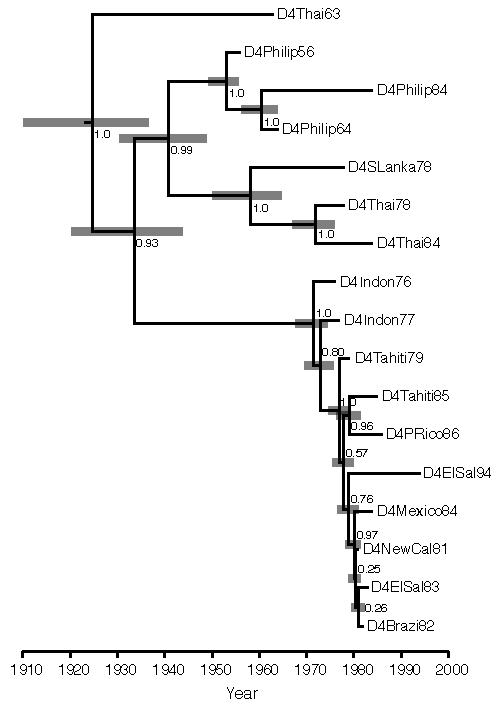
\includegraphics{fig01.pdf}}
\caption{The consensus tree for the Dengue 4 sequences. Each internal node is labeled with the posterior probability of monophyly of the corresponding clade. The gray bars illustrated the extent of the 95\% highest posterior density intervals for each divergence time. The scale is in years. }\label{fig:01}
\end{figure}


\section{Results and Discussion}

BEAST provides considerable flexibility in the specification of an
evolutionary model. For example, consider the analysis of a multiple
sequence alignment of coding DNA. In a BEAST analysis, it is possible
to allow each codon position to have a different rate, a different
amount of rate heterogeneity among sites, and a different amount of
rate heterogeneity among branches, while, at the same time, sharing
the same intrinsic ratio of transitions to transversions with the
other codon positions. In fact, all parameters can be shared or made
independent among partitions of the sequence data. 

An unavoidable feature of Bayesian statistical analysis is the specification
of a prior distribution over parameter values. This requirement is
both an advantage and a burden. It is an advantage because relevant
knowledge such as palaeontological calibration of phylogenies is readily
incorporated into an analysis. However, when no obvious prior distribution
for a parameter exists, a burden is placed on the researcher to ensure
that the prior selected is not inadvertently influencing the posterior
distribution of parameters of interest.

In BEAST, all parameters (whether they be substitutional, demographic or genealogical)
can be given informative priors (e.g. exponential, normal, lognormal
or uniform with bounds, or combinations of these). For example, the age of the root of the tree
can be given an exponential prior with a pre-specified mean. 

The five components of an evolutionary model for a set of aligned
nucleotides in BEAST are: 

\begin{itemize}
\item Substitution model - The substitution model is a homogeneous Markov
process that defines the relative rates at which different substitutions
occur along a branch in the tree.
\item Rate model among sites - The rate model among sites defines the distribution
of relative rates of evolutionary change among sites.
\item Rate model among branches - The rate model among branches defines
the distribution of rates among branches and is used to convert the
tree, which is in units of time, to units of substitutions. These
models are important for divergence time estimation procedures.
\item Tree - a model of the phylogenetic or genealogical relationships of
the sequences.
\item Tree prior - The tree prior provides a parameterized prior distribution
for the node heights (in units of time) and tree topology. 
\end{itemize}

\subsection*{Substitution models and rate models among sites}

For nucleotide data, all of the models that are nested in the general
time-reversible (GTR) model \citep{ROMM1990} - including the well
known HKY85 model \citep{ha85} - can be specified. For the analysis
of amino acid sequence alignments all of the following replacement
models can be used: Blosum62, CPREV, Dayhoff, JTT, MTREV and WAG.
When nucleotide data represents a coding sequence (i.e. an in-frame
protein-coding sequence with introns removed) the Goldman and Yang model \citep{goldman94} can be used to model
codon evolution. 

In addition, both $\Gamma$-distributed rates among sites \citep{yang94approx}
and a proportion of invariant sites can be used to describe rate heterogeneity
among sites.


\subsection*{Rate models among branches, divergence time estimation and time-stamped
data}

The basic model for rates among branches supported by BEAST is the
strict molecular clock model \citep{zuckerkandl65}, calibrated by specifying
either a substitution rate or the date of a node or set of nodes.
In this context, dates of divergence for particular clades can be
estimated. The clades can be defined either by a monophyletic grouping
of taxa or as the most recent common ancestor of a set of taxa of
interest. The second alternative does not require monophyly of the
selected taxa with respect to the rest of the tree. Furthermore, when
the differences in the dates associated with the tips of the tree
comprise a significant proportion of the age of the entire tree, these
dates can be incorporated into the model providing a source of information
about the overall rate of evolutionary change \citep{drummond02, drummond03}.

In BEAST, divergence time estimation has also been extended to include
\emph{relaxed phylogenetics} models, in which the rate of evolution
is allowed to vary among the branches of the tree. In particular we
support a class of uncorrelated relaxed clock branch rate models,
in which the rate at each branch is drawn from an underlying distribution
such as exponential or lognormal \citep{drummond06}.

If the sequence data are all from one time point, then the overall
evolutionary rate must be specified with a strong prior. The units
implied by the prior on the evolutionary rate will determine the units
of the node heights in the tree (including the age of the most recent
common ancestor) as well as the units of the demographic parameters
such as the population size parameter and the growth rate. For example,
if the evolutionary rate is set to 1.0, then the node heights (and
root height) will be in units of mutations per site (i.e. the units
of branch lengths produced by common software packages such as \textbf{\textsc{MrBayes}}
3.0). Similarly, for a haploid population, the coalescent parameter
will be an estimate of $N_{e}\mu$. However, if, for example, the
evolutionary rate is expressed in mutations per site per year, then
the branches in the tree will be in units of years. Furthermore the
population size parameter of the demographic model will then be equal
to $N_{e}\tau$, where $N_{e}$ is the effective population size and
$\tau$ is the generation length in years. Finally, if the evolutionary
rate is expressed in units of mutations per site per generation then
the resulting tree will be in units of generations and the population
parameter of the demographic model will be in natural units (i.e.
will be equal to the effective number of reproducing individuals,
$N_{e}$).


\subsection*{Tree Priors}

When sequence data has been collected from a homogenous population,
various coalescent \citep{Kingman1982,GT1994} models of demographic
history can be used in BEAST to model population size changes through
time. At present the simple parametric models available include constant
size $N(t)=N_{e}$ (1 parameter), exponential growth $N(t)=N_{e}e^{-gt}$
(2 parameters) and logistic growth (3 parameters). 

In addition, the highly parametric Bayesian skyline plot \citep{drummond05}
is also available, but this model can only be used when the data are
strongly informative about population history. All of these demographic
models are parametric priors on the ages of nodes in the tree, in
which the hyperparameters (e.g., population size, $N_{e}$, and growth
rate, $g$) can be sampled and estimated. As well as performing single
locus coalescent-based inference, two or more unlinked gene trees
can be simultaneously analyzed under the same demographic model. Sophisticated
multi-locus coalescent inference can be achieved by allocating a separate
overall rate and substitution process for each locus, thereby accommodating
loci with heterogeneous evolutionary processes.

At present there are only a limited number of options for non-coalescent
priors on tree shape and branching rate. Currently a simple Yule prior
on birth rate of new lineages (1 parameter) can be employed. However,
generalized birth-death tree priors are currently under development.

In addition to general models of branching times such as the coalescent
and Yule priors, the tree prior may also include specific distributions
and/or constraints on certain node heights and topological features.
These additional priors may represent other sources of knowledge such
as expert interpretation of the fossil record. For example, as briefly
noted above, each node in the tree can have a prior distribution representing
knowledge of its date. A recent paper on ``relaxed phylogenetics''
contains more information on calibration priors \citep{drummond06}. 


\subsection*{Insertion-deletion models}

Finally, BEAST also has a model of the insertion-deletion process.
This provides the ability to co-estimate the phylogeny and the multiple
sequence alignment. Currently only the TKF91 model of insertion-deletion
\citep{thorne91} is available. Interested readers should refer to the
paper on this subject for more details \citep{lunter05}.


\subsection*{Multiple data partitions and linking and unlinking parameters}

BEAST provides the ability to analyze multiple data partitions simultaneously.
This is useful when combining multiple genes in a single multi-locus
coalescent analysis (e.g. \citep{Lemeyetal2004}) or to allocate different
evolutionary processes to different regions of a sequence alignment
(such as the codon positions; e.g. \citep{PDNRR2003}). The parameters
of the substitution model, the rate model among sites, the rate model
among branches, the tree, and the tree prior can all be 'linked' or
'unlinked' in a analysis involving multiple partitions. For example
in an analysis of HIV-1 group O by Lemey \emph{et al} \citep{Lemeyetal2004},
three loci (gag, int, pol) were assumed to share the same substitution
model parameters (GTR), as well as sharing the same demographic history
of exponential growth. However they were assumed to have different
shape parameters for $\Gamma$-distributed rate heterogeneity among
sites, different rate parameters for the strict molecular clock and
the three tree topologies and sets of divergence times were also assumed
to be independent and unlinked. 

\subsection*{Definitions and units of the standard parameters}

Crucial to the interpretation of all BEAST parameters is an understanding of the units that the tree is measured in. The
simplest situation occurs when no calibration information is available, either from knowledge of the rate of evolution
of the gene region, or from knowledge of the age of any of the nodes in the tree. If this is the case the rate of
evolution is set to 1.0 and the branch lengths in the tree are then in substitutions per site. However if the rate of
evolution is known in substitutions per site per unit time, then the genealogy will be expressed in the relevant time
units. Likewise, if the age of one or more nodes (internal or external) are known then this will also provide the units
for the rest of the branch lengths and the rate of evolution. Note that only the set of parameters that are currently
being used (as defined by the model settings) will be shown in the table. For example, if the rate of substitution is
fixed (in the ``Model'' section) then the \xml{clock.rate} parameter (or the  \xml{ucld.mean} if the relaxed clock
is selected) will not be available. With this in mind, the following table lists some of the parameters that can be
generated by BEAUti, their interpretation and units.

\begin{lyxlist}{00.00.0000000000000000}
\item [\texttt{\small{clock.rate}}] The rate of the strict molecular clock. This parameter only appears when you have
selected the strict molecular clock in the model panel. The units of this parameter are in substitutions per site per
unit time. If this parameter is fixed to 1.0 (using the {\it Fix mean substitution rate} option in the Model panel) then
the branch lengths in the tree will be in units of substitutions per site. However, if, for example, the tree is being
calibrated by using fossil calibrations on internal nodes and those fossil dates are expressed in millions of years ago
(Mya), then the \texttt{clock.rate} parameter will be an estimate of the evolutionary rate in units of substitutions
per site per million years (Myr).

\item [\texttt{\small{constant.popSize}}] This is the coalescent parameter under the assumption of a constant population
size. This parameter only appears if you select a constant size coalescent tree prior. This parameter represents the
product of effective population size ($N_e$) and the generation length in units of time ($\tau$). If time is measured in
generations this parameter a direct estimate of $N_e$. Otherwise it is a composite parameter and an estimate of $N_e$
can be computed from this parameter by dividing it by the generation length in the units of time that your calibrations
(or \xml{clock.rate}) are defined in. Finally,  if \xml{clock.rate} is set to $1.0$ then \xml{constant.popSize} is an
estimate of $N_e\mu$ for haploid data such as mitochondrial sequences and $2N_e\mu$ for diploid data, where $\mu$ is the
substitution rate per site per generation.

\item [\texttt{\small{covariance}}] If this value is significantly positive, then it means that within your phylogeny,
branches with fast rates are followed by branches with fast rates. This statistic measures the covariance between parent
and child branch rates in your tree in a relaxed molecular clock analysis. If this value spans zero, then branches with
fast rates and slow rates are next to each other.  It also means that there is no strong evidence of autocorrelation
of rates in the phylogeny.

\item [\texttt{\small{exponential.growthRate}}]	 This is the coalescent parameter representing the rate of growth of the
population assuming exponential growth. The population size at time $t$ is determined by $N(t)=N_e\exp(-gt)$ where $t$
is in the same units as the branch lengths and $g$ is the \xml{exponential.growthRate} parameter. This parameter only
appears if you have selected a exponential growth coalescent tree prior.

\item [\texttt{\small{exponential.popSize}}]	 This is the parameter representing the modern day population size
assuming exponential growth. Like \xml{constant.popSize}, it is a composite parameter unless the time scale of the
genealogy is in generations. This parameter only appears if you have selected a exponential growth coalescent tree
prior.

\item [\texttt{\small{gtr.\{ac,ag,at,cg,gt\}}}]	 These five parameters are the relative rates of substitutions for
$A{\leftrightarrow}C$,  $A{\leftrightarrow}G$,  $A{\leftrightarrow}T$,  $C{\leftrightarrow}G$ and  $G{\leftrightarrow}T$
in the general time-reversible model of nucleotide substitution \citep{ROMM1990}. In the default set up these parameters
are relative to $r_{C{\leftrightarrow}T} = 1.0$. These parameters only appear if you have selected the GTR substitution
model.

\item [\texttt{\small{hky.kappa}}]	 This parameter is the transition/transversion ratio ($\kappa$) parameter of the
HKY85 model of nucleotide substitution \citep{ha85}. This parameter only appears if you have selected the HKY
substitution model.

\item [\texttt{\small{siteModel.alpha}}]	 This parameter is the shape ($\alpha$) parameter of the $\Gamma$
distribution of rate heterogeneity among sites \citep{yang94approx}. This parameter only appears when you have selected Gamma
or Gamma+Invariant Sites in the site heterogeneity model.

\item [\texttt{\small{siteModel.pInv}}]	 This parameter is the proportion of  invariant sites ($p_{inv}$) and has a
range between 0 and 1. This parameter only appears when you have selected ``Invariant sites'' or ``Gamma+Invariant Sites'' in
the site heterogeneity model. The starting value must be less than 1.0.

\item [\texttt{\small{treeModel.rootHeight}}]	 This parameter represents the total height of the tree (often known as
the $t_{MRCA}$). The units of this variable are the same as the units for the branch lengths in the tree and will depend on the calibration information for the rate and/or dates of calibrated nodes.

\item [\texttt{\small{ucld.mean}}]	 This is the mean molecular clock rate under the uncorrelated lognormal relaxed
molecular clock. This parameter can be in real space or in log space depending on the BEAST XML. However,under default
BEAUti options for the uncorrelated log-normal relaxed clock this parameter has the same units as \xml{clock.rate}.
\item [\texttt{\small{ucld.stdev}}] This is the standard deviation ($\sigma$) of the uncorrelated lognormal relaxed
clock (in log-space). If this parameter is 0 there is no variation in rates among branches. If this parameter is greater
than 1 then the standard deviation in branch rates is greater than the mean rate. This is also the case for the
coefficient of variation.  When viewed in Tracer, if the coefficient of variation frequency histogram is abutting
against zero, then your data can't reject a strict molecular clock.  If the frequency histogram is not abutting against
zero then there is among branch rate heterogeneity within your data, and we recommend the use of a relaxed molecular
clock.

\item [\texttt{\small{yule.birthRate}}]	This parameter is the rate of lineage birth in the Yule model of speciation. If
\xml{clock.rate} is 1.0 then this parameter estimates the number of lineages born from a parent lineage per substitution
per site. If the tree is instead measured in, for example, years, then this parameter would be the number of new lineages
born from a single parent lineage per year.

\item [\texttt{\small{tmrca({\it taxon group})}}]	This is the parameter for the $t_{MRCA}$ of the specified taxon
subset that you specified in the ``Taxa'' panel. The units of this variable are the same as the units for the branch
lengths in the tree and will depend on the calibration information for the rate and/or dates of calibrated nodes.  There
will a \xml{tmrca({\it taxon group})} parameter for each taxon subset specified. Setting priors on these parameters
and/or \xml{treeModel.rootHeight} parameter will act as calibration information.
\end{lyxlist}

\section{Conclusions}

BEAST is a flexible analysis package for evolutionary parameter estimation
and hypothesis testing. The component-based nature of model specification
in BEAST means that the number of different evolutionary models possible
is very large and therefore difficult to summarize. However a number
of published uses of the BEAST software already serve to highlight
the breadth of application the software enjoys \citep{PDNRR2003,Lemeyetal2004,Shapiroetal2004,drummond05, lunter05}. 

BEAST is an actively developed package and enhancements for the next
version include (1) birth-death priors for tree shape (2) faster and
more flexible codon-based substitution models (3) the structured coalescent
to model subdivided populations with migration (4) models of continuous
character evolution and (5) new relaxed clock models based on random local molecular clocks. 


\section*{Availability and Requirements}

\begin{itemize}
\item Project name: BEAST (Bayesian evolutionary analysis sampling trees)
\item Project home page: http://code.google.com/p/beast-mcmc/
\item Operating system(s): Platform independent
\item Programming language: Java and C 
\item Other requirements: Java 1.4 or higher
\item License: GNU LGPL
\item Any restrictions to use by non-academics: for-profit organisations
should contact authors for licensing arrangements. 
\end{itemize}

\section*{List of Abbreviations}

\begin{lyxlist}{00.00.0000}
\item [{\textsc{BEAST}}] \textsc{Bayesian evolutionary analysis sampling
trees}
\item [{\textsc{HKY85}}] \textsc{Hasegawa-Kishino-Yano 1985}
\item [{\textsc{GTR}}] \textsc{general time-reversible}
\item [{\textsc{MCMC}}] \textsc{Markov chain Monte Carlo}
\item [{\textsc{TKF91}}] \textsc{Thorne-Kishino-Felsenstein 1991}
\end{lyxlist}

\section*{Authors Contributions}

AJD and AR designed and implemented all versions of BEAST up to the
current (version 1.4), which was developed between June 2002 and June
2007. Portions of the BEAST source code are based on an original Markov
chain Monte Carlo program developed by AJD (called MEPI) during his
PhD at Auckland University between the years 2000 and 2002. Portions
of the BEAST source code are based on previous C++ software developed
by AR. Both authors contributed to the writing of this paper.


\section*{Acknowledgements}

We would like to thank Roald Forsberg, Joseph Heled, Gerton Lunter, Sidney Markowitz, 
Oliver Pybus, Beth Shapiro, Korbinian Strimmer and Marc Suchard for invaluable contributions. 
AJD was partially supported by the Wellcome Trust and AR was supported
by the Royal Society.


\bibliographystyle{plainnat}
\bibliography{BEAST}




\end{document}
